\definecolor{qqwuqq}{rgb}{0.,0.39215686274509803,0.}
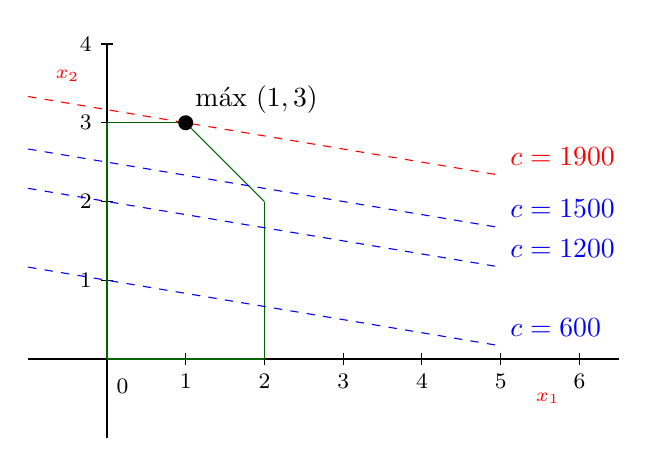
\begin{tikzpicture}[x=1.0cm,y=1.0cm]
\draw[color=black] (-1,0) -- (6.5,0);
\foreach \x in {1,2,3,4,5,6}
\draw[shift={(\x,0)},color=black] (0pt,2pt) -- (0pt,-2pt) node[below] {\footnotesize $\x$};
\draw[color=black] (0,-1) -- (0,4);
\foreach \y in {1,2,3,4}
\draw[shift={(0,\y)},color=black] (2pt,0pt) -- (-2pt,0pt) node[left] {\footnotesize $\y$};
\draw[color=black] (0pt,-10pt) node[right] {\footnotesize $0$};

\draw [color=qqwuqq] (0.,3.)-- (1.,3.);
\draw [color=qqwuqq] (1.,3.)-- (2.,2.);
\draw [color=qqwuqq] (2.,2.)-- (2.,0.);
\draw [color=qqwuqq] (2.,0.)-- (0.,0.);
\draw [color=qqwuqq] (0.,0.)-- (0.,3.);

\draw [domain=-1.:5, color = blue, dashed] plot(\x,{2.5-(\x/6)}) node[anchor=south west] {$c = 1500$};
\draw [domain=-1.:5, color = blue, dashed] plot(\x,{2-(\x/6)}) node[anchor=south west] {$c = 1200$};
\draw [domain=-1.:5, color = blue, dashed] plot(\x,{1-(\x/6)}) node[anchor=south west] {$c = 600$};
\draw [domain=-1.:5, color = red, dashed] plot(\x,{3.166666667-(\x/6)}) node[anchor=south west] {$c = 1900$};

\draw [fill=black] (1,3) circle(2.5pt) node [anchor = south west] {máx $(1,3)$};

\begin{scriptsize}
\draw[color=red] (5.6, -0.5) node {$x_1$};
\draw[color=red] (-0.5,3.6) node {$x_2$};
\end{scriptsize}
\end{tikzpicture}